%!TeX encoding = UTF-8
%!TeX program = xelatex
\documentclass[
  notheorems,
  aspectratio=54,
]{beamer}

%% preamble
\title{An Introduction to Synchronization on Complex Networks}
% \subtitle{The subtitle}
\author{Jingsheng Gao}
\institute{Anqing Normal University}

\useoutertheme{shadow}
\setbeamertemplate{headline}{}
\mode<presentation>{
  \usetheme{Warsaw}
  \usecolortheme{seagull}
}

\setbeamertemplate{footline}
{
  \leavevmode%
  \hbox{%
  \begin{beamercolorbox}[wd=.45\paperwidth,ht=2.25ex,dp=1ex,center]{title in head/foot}%
    \usebeamerfont{title in head/foot}\inserttitle
  \end{beamercolorbox}%
  \begin{beamercolorbox}[wd=.45\paperwidth,ht=2.25ex,dp=1ex,center]{author in head/foot}%
      \usebeamerfont{author in head/foot}\insertauthor\ - \insertinstitute
  \end{beamercolorbox}%
  \begin{beamercolorbox}[wd=.1\paperwidth,ht=2.25ex,dp=1ex,right]{date in head/foot}%
    \insertframenumber{} / \inserttotalframenumber\hspace*{2ex} 
  \end{beamercolorbox}}%
  \vskip0pt%
}


\setbeamertemplate{navigation symbols}{}

\usepackage[
    backend=biber,
    autocite=superscript,
    sorting=none
]{biblatex}
\AtBeginBibliography{\small}
\addbibresource{refs.bib}

\usepackage{caption}
\captionsetup[figure]{font=scriptsize}

\usepackage{latexsym}
\usepackage{amsmath,amssymb}
\usepackage{mathtools}
\usepackage{color,xcolor}
\usepackage{graphicx}
\usepackage{algorithm}
\usepackage{amsthm}
\usepackage{lmodern}
% \usepackage[UTF8]{ctex}
% \usepackage{xeCJK}
\usepackage{animate} % insert gif

\usepackage{lipsum}
\usepackage{ulem}

\usepackage{listings} % display code on slides; don't forget [fragile] option after \begin{frame}

% ----------------------------------------------
% tikx
\usepackage{framed}
\usepackage{tikz}
\usepackage{pgf}
\usetikzlibrary{calc,trees,positioning,arrows,chains,shapes.geometric,%
    decorations.pathreplacing,decorations.pathmorphing,shapes,%
    matrix,shapes.symbols}



% ----------------------------------------------

% ---------------------------------------------------------------------
% Jet Black Theme
% \setbeamercolor{normal text}{fg=white,bg=black!90}
% \setbeamercolor{structure}{fg=white}
%
% \setbeamercolor{alerted text}{fg=red!85!black}
%
% \setbeamercolor{item projected}{use=item,fg=black,bg=item.fg!35}
%
% \setbeamercolor*{palette primary}{use=structure,fg=structure.fg}
% \setbeamercolor*{palette secondary}{use=structure,fg=structure.fg!95!black}
% \setbeamercolor*{palette tertiary}{use=structure,fg=structure.fg!90!black}
% \setbeamercolor*{palette quaternary}{use=structure,fg=structure.fg!95!black,bg=black!80}
%
% \setbeamercolor*{framesubtitle}{fg=white}
%
% \setbeamercolor*{block title}{parent=structure,bg=black!70!gray}
% \setbeamercolor*{block body}{fg=black,bg=black!10}
% \setbeamercolor*{block title alerted}{parent=alerted text,bg=black!15}
% \setbeamercolor*{block title example}{parent=example text,bg=black!15}
% ---------------------------------------------------------------------


% \newcommand{\reditem}[1]{\setbeamercolor{item}{fg=red}\item #1}

% \newcommand*{\Scale}[2][4]{\scalebox{#1}{\ensuremath{#2}}}

% -------------------------------------------------------------

% -------------------------------------------------------------

\begin{document}

% title frame
\begin{frame}
    \titlepage
\end{frame}

\begin{frame}{Introduction}
 \begin{itemize}
    \item Synchronization on complex networks is a fascinating phenomenon that explores how interconnected systems can achieve coordinated behavior.
    \item Among collective phenomena in natural and social systems, the synchronization of a set of interacting individuals or units has been intensively studied because of its ubiquity in the natural world.
    \item It is applied on engineering systems, biological systems, social dynamics, and more
  \end{itemize}
\end{frame}

\begin{frame}{1. Synchronization}
  \begin{figure}
    \centering
  \end{figure}
  \begin{itemize}
    \item Synchronization is the process by which components of a system adjust their behavior to a common rhythm or pattern.
    \item Metronome synchronization, firefly flashing, circadian rhythms, brain networks.
\begin{figure}
  \begin{minipage}[b]{0.45\textwidth}
    \textbf{Schooling Fish}\par\medskip
    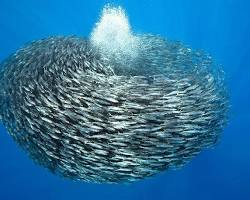
\includegraphics[width=0.4\textwidth]{schooling_fish.png}
  \end{minipage}
  \hfill
  \begin{minipage}[b]{0.45\textwidth}
    \textbf{Bioluminescence in Oceans}\par\medskip
    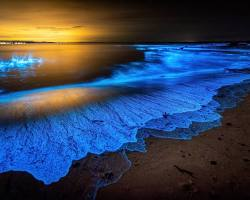
\includegraphics[width=0.4\textwidth]{bioluminescence.png}
  \end{minipage}
\end{figure}
  \end{itemize}
\end{frame}


\begin{frame}{2. Complex Networks}
  \begin{itemize}
    \item A complex network is a graph (network) with non-trivial topological features—features that do not occur in simple networks such as lattices or random graphs but often occur in networks representing real systems.
    \item  The study of complex networks is a young and active area of scientific research (since 2000) inspired largely by empirical findings of real-world networks such as computer networks, biological networks, technological networks, brain networks, climate networks and social networks.
  \end{itemize}
\end{frame}

\begin{frame}{3. Factors Influencing Synchronization}
  \begin{itemize}
    \item Network Topology: The structure of connections, such as of small-world network, scale-free network, Erdős–Rényi model, significantly impacts synchronization.
    \item Coupling Strength: The intensity of interactions between nodes plays a crucial role. Stronger coupling generally promotes synchronization.
    \item Node Dynamics: The intrinsic properties of individual nodes, such as their natural frequencies or response patterns, also influence synchronization.
  \end{itemize}
\end{frame}

\begin{frame}{3.1 Scale-free network}
  \begin{itemize}
   \item A scale-free network\cite{wiki:scale_free_network} is a network whose degree distribution follows a power law, at least asymptotically.
  \end{itemize}
  \begin{figure}
    \centering
    \textbf{Examples}\par\medskip
    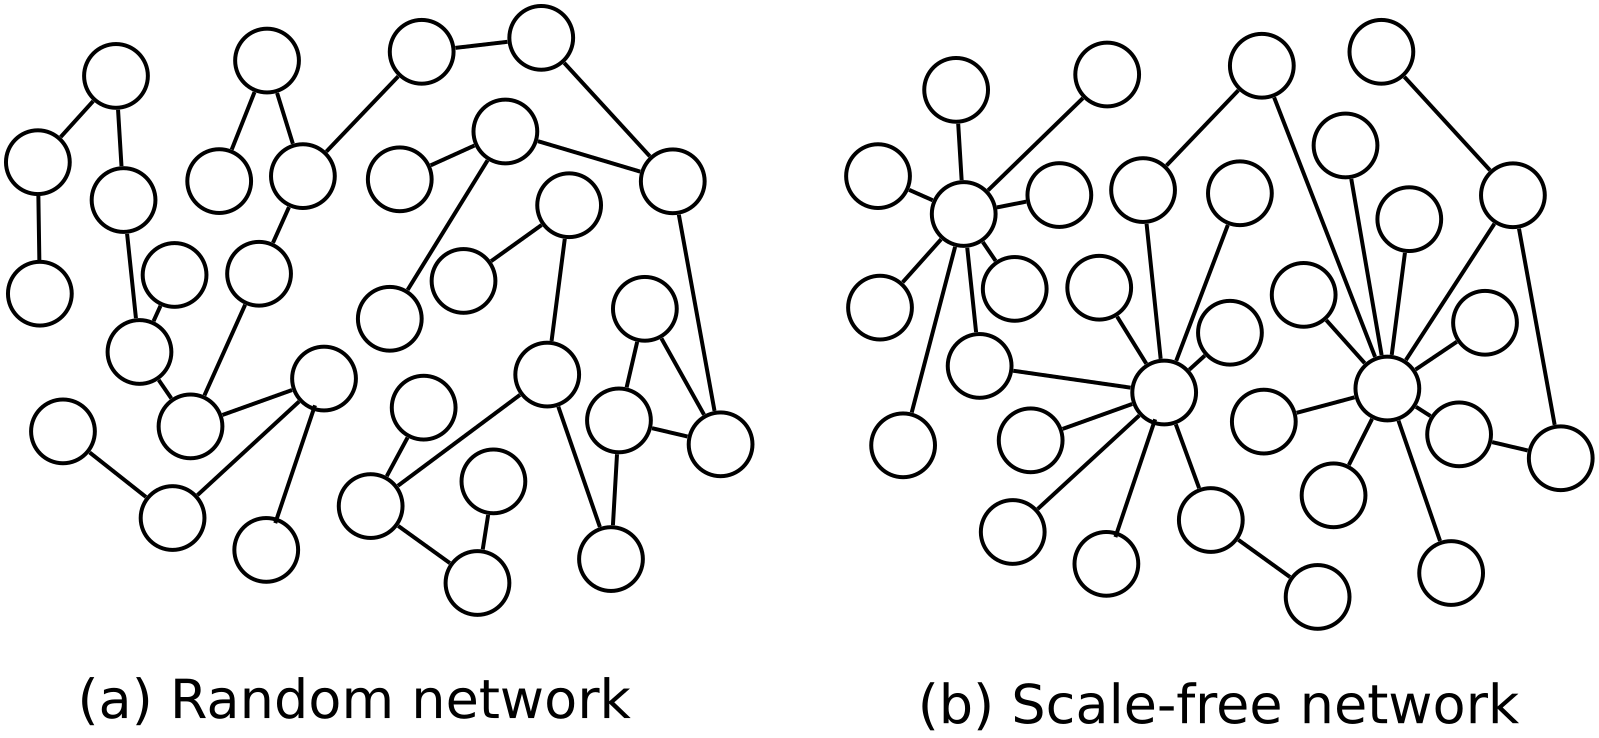
\includegraphics[width=0.4\textwidth]{scale_free_network.png}
  \end{figure}
  \begin{figure}
    \centering
    \textbf{Degree distribution}\par\medskip
    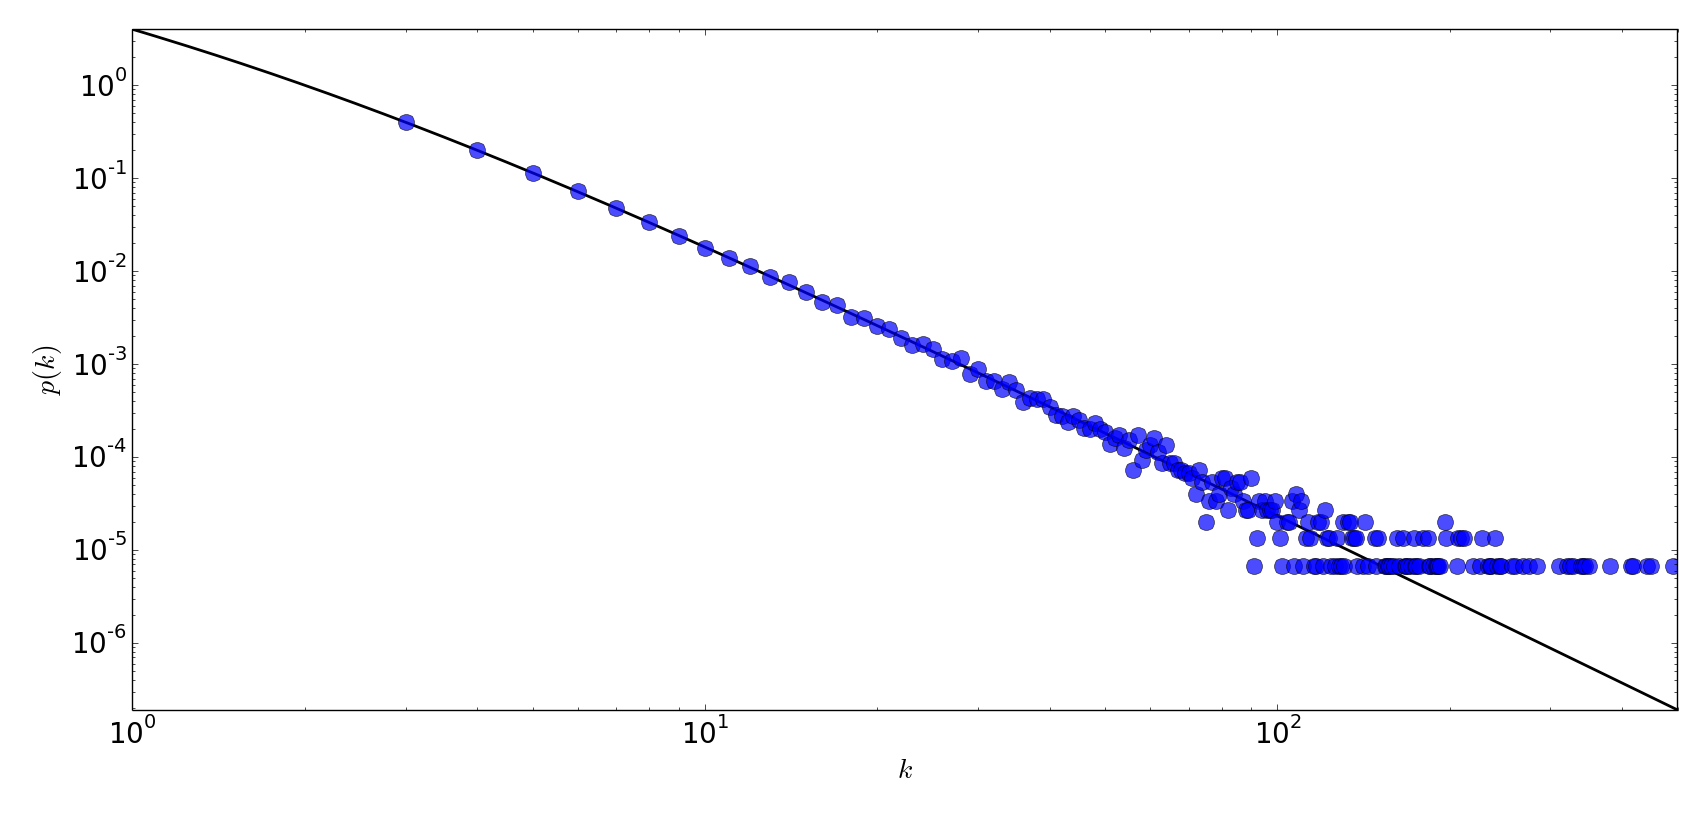
\includegraphics[width=0.4\textwidth]{scale_free_distribution.png}
    \caption{Degree distribution for a network with 150000 vertices and mean degree = 6 created using the Barabási–Albert model (blue dots). The distribution follows an analytical form given by the ratio of two gamma functions (black line) which approximates as a power-law.}
  \end{figure}
\end{frame}

\begin{frame}{3.2 Erdős–Rényi model}
  \begin{itemize}
      \item In the mathematical field of graph theory, the Erdős–Rényi model\cite{wiki:er_model} refers to one of two closely related models for generating random graphs or the evolution of a random network.
  \end{itemize}
  \begin{figure}
    \centering
    \textbf{Partial map of the Internet}\par\medskip
    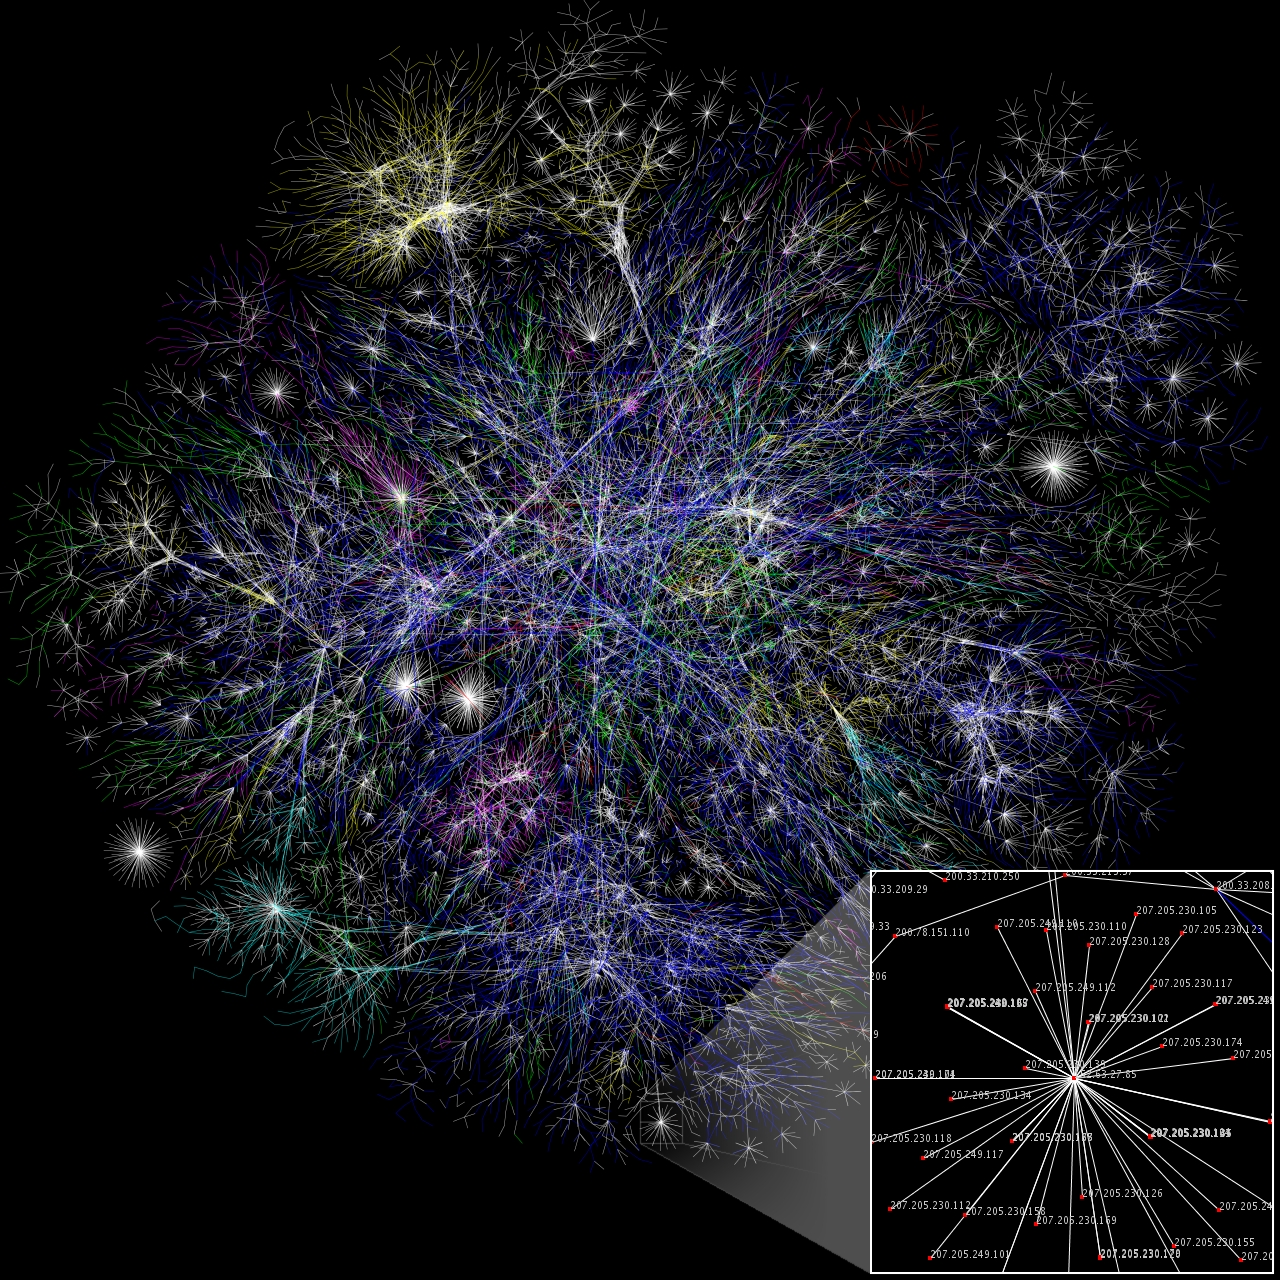
\includegraphics[width=0.4\textwidth]{internet_map.jpg}
      \caption{Each line is drawn between two nodes, representing two IP addresses. The length of the lines are indicative of the delay between those two nodes. This graph represents less than 30\% of the Class C networks reachable by the data collection program in early 2005.}
  \end{figure}
\end{frame}

\begin{frame}{3.2 Generating methods of Erdős–Rényi model}
  \begin{itemize}
    \item In the $G(n, M)$ model, a graph is chosen uniformly at random from the collection of all graphs which have $n$ nodes and M edges. For example, in the $G(3,2)$ model, there are three two-edge graphs on three labeled vertices (one for each choice of the middle vertex in a two-edge path), and each of these three graphs is included with probability.
    \item In the $G(n, p)$ model, a graph is constructed by connecting labeled nodes randomly. Each edge is included in the graph with probability $p$, independently from every other edge. Equivalently, the probability for generating each graph that has $n$ nodes and $M$ edges is ${\displaystyle p^{M}(1-p)^{{n \choose 2}-M}}$.
  \begin{figure}
    \centering
    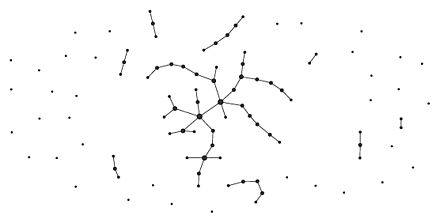
\includegraphics[width=0.4\textwidth]{er_example.jpg}
    \caption{A graph generated by the binomial model of Erdős and Rényi (p = 0.01)}
  \end{figure}
  \end{itemize}
\end{frame}

\begin{frame}{4. Models and analysis}
  \begin{itemize}
    \item The Kuramoto model, first proposed by Yoshiki Kuramoto, is a nonlinear dynamic system used in describing synchronization of coupled oscillators that initially have random natural frequencies and phases.
    \item In mathematics, the master stability function is a tool used to analyze the stability of the synchronous state in a dynamical system consisting of many identical systems which are coupled together, such as the Kuramoto model.
  \end{itemize}
\end{frame}

\begin{frame}{4.1 Nonlinear system}
  In mathematics, a linear map (or linear function) $f(x)$ is one which satisfies both of the following properties:
  \begin{itemize}
    \item Additivity or superposition principle: ${\displaystyle \textstyle f(x+y)=f(x)+f(y)}$;
    \item Homogeneity: ${\displaystyle \textstyle f(\alpha x)=\alpha f(x)}$.
  \end{itemize}
  An equation written as $f(x)=C$ is called linear if $f(x)$ is a linear map (as defined above) and nonlinear otherwise.
\end{frame}

\begin{frame}{4.1 Nonlinear system}
  \begin{itemize}
    \item System of linear differential equations:
    ${\displaystyle {\begin{aligned}y_{1}'(x)&=b_{1}(x)+a_{1,1}(x)y_{1}+\cdots +a_{1,n}(x)y_{n}\\[1ex]&\;\;\vdots \\[1ex]y_{n}'(x)&=b_{n}(x)+a_{n,1}(x)y_{1}+\cdots +a_{n,n}(x)y_{n}\end{aligned}}}$
    \\ where $b_{n}$ and the $a_{i,j}$ are functions of x. In matrix notation, this system may be written
${\displaystyle \mathbf {y} '=A\mathbf {y} +\mathbf {b}}$.
    \item A system of differential equations is said to be nonlinear if it is not a system of linear equations. For example:
  \\\centering ${\frac  {d\theta _{i}}{dt}}=\omega _{i}+{\frac  {K}{N}}\sum _{{j=1}}^{{N}}\sin(\theta _{j}-\theta _{i}),\qquad i=1\ldots N$.
  \end{itemize}
\end{frame}


\begin{frame}{4.2 Kuramoto model}
  In the most popular version of the Kuramoto model, each of the oscillators is considered to have its own intrinsic natural frequency
  $\omega _{i}$, and each is coupled equally to all other oscillators.
  The most popular form of the model has the following governing equations:
  \\\centering ${\frac  {d\theta _{i}}{dt}}=\omega _{i}+{\frac  {K}{N}}\sum _{{j=1}}^{{N}}\sin(\theta _{j}-\theta _{i}),\qquad i=1\ldots N$,
  \\\raggedright where the system is composed of N limit-cycle oscillators, with phases ${\displaystyle \theta _{i}}$ and coupling constant K.
  \begin{figure}
    \centering
    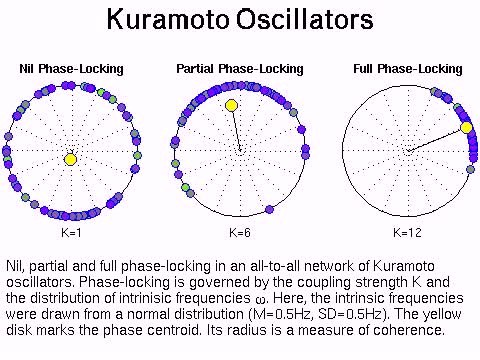
\includegraphics[width=0.6\textwidth]{kuramoto_oscilators.jpg}
  \end{figure}
\end{frame}

\begin{frame}{4.2.1 Coupled oscillations}
  \begin{figure}
    \centering
    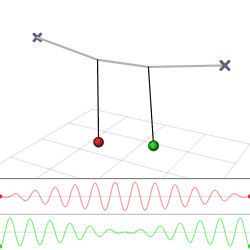
\includegraphics[width=0.6\textwidth]{Coupled_oscillators.png}
    \caption{Two pendulums with the same period fixed on a string act as pair of coupled oscillators. The oscillation alternates between the two.}
  \end{figure}
\end{frame}

\begin{frame}{References}
    \printbibliography
\end{frame}

\begin{frame}{}
  \centering \Huge
  \emph{Thanks for listening!}
\end{frame}

\end{document}



